\documentclass[12pt]{article}
\usepackage[utf8]{inputenc}
% Deutsch: https://de.overleaf.com/learn/German
% "`	Left double quotes
% "'	Right double quotes
\usepackage[T1]{fontenc}
\usepackage[ngerman]{babel}
\usepackage{csquotes}

\usepackage{xcolor}
\usepackage{listings}

\definecolor{mGreen}{rgb}{0,0.6,0}
\definecolor{mGray}{rgb}{0.5,0.5,0.5}
\definecolor{mPurple}{rgb}{0.58,0,0.82}
\definecolor{backgroundColour}{rgb}{0.95,0.95,0.92}

\lstdefinestyle{CStyle-numbers}{
    backgroundcolor=\color{backgroundColour},   
    commentstyle=\color{mGreen},
    keywordstyle=\color{magenta},
    numberstyle=\tiny\color{mGray},
    stringstyle=\color{mPurple},
    basicstyle=\footnotesize,
    breakatwhitespace=false,         
    breaklines=true,                 
    captionpos=b,                    
    keepspaces=true,                 
    numbers=left,                    
    numbersep=5pt,                  
    showspaces=false,                
    showstringspaces=false,
    showtabs=false,                  
    tabsize=2,
    language=C
}

\lstdefinestyle{CStyle}{
    backgroundcolor=\color{backgroundColour},   
    commentstyle=\color{mGreen},
    keywordstyle=\color{magenta},
    stringstyle=\color{mPurple},
    basicstyle=\footnotesize,
    breakatwhitespace=false,         
    breaklines=true,                 
    captionpos=b,                    
    keepspaces=true,                         
    showspaces=false,                
    showstringspaces=false,
    showtabs=false,                  
    tabsize=2,
    language=C
}

\usepackage{tikz}
\usetikzlibrary{positioning,automata}

\usepackage[acronym,nonumberlist]{glossaries}
\usepackage{acronym}

% documentation: https://ctan.kako-dev.de/macros/latex/contrib/biblatex/doc/biblatex.pdf
\usepackage[backend=biber,style=numeric,sorting=ynt]{biblatex}
\addbibresource{references.bib}

% um Grafiken einzubinden, {Angabe des Pfades der Bilder}
\usepackage{float}
\usepackage{graphicx}
\graphicspath{ {images/} }
% Nützliches Online Tool zur Tabellengenerierung: TablesGenerator.com 

% zur korreten Platzierung der Bilder im Titelblatt
\usepackage{chngpage}
\usepackage{calc}
\usepackage{geometry}

% Automatisches Generieren von Hyperlinks bei Verweisen (ref / cite)
\usepackage{hyperref}
\hypersetup{
  colorlinks   = true,    % Colours links instead of ugly boxes
  urlcolor     = blue,    % Colour for external hyperlinks
  linkcolor    = black,    % Colour of internal links
  citecolor    = red      % Colour of citations
}

% Infos über Dokument
\title{Arduino Projekt}
\author{Sebastian Pötter}
\date{\today}

\begin{document}

    \newgeometry{top=2cm,bottom=2cm}

\begin{titlepage}
    
    \begin{figure}[t]
        \begin{adjustwidth}{-\oddsidemargin-1in}{-\rightmargin}
            \centering
            
\includegraphics[width=\paperwidth]{banner_top}
        \end{adjustwidth}
    \end{figure}

    \begin{flushleft}
        \vspace*{1cm}
        \Huge
        \textbf{Projekt für Embedded Systems}
        
        \vspace{0.5cm}
        \LARGE
        Schlosssteuerung mit LED und Keypad
        
        \vspace{1.5cm}
        \textbf{Lukas Brüggemann, Markus Reinhold, Sebastian Pötter}
        
        \vspace{0.5cm}
        \large
        Jahrgang: 20INM
        
        \vspace{0.5cm}
        im Studiengang\\
        Informatik Master
        
    \end{flushleft}        

    \vspace{0.5cm}
    \begin{flushright}
        Embedded Systems (7320)\\
        Prof. Dr.-Ing. Andreas Pretschner\\
        \vspace{0.5cm}
        \today
    \end{flushright}    
    
    \begin{figure}[b]
        \begin{adjustwidth}{-\oddsidemargin-1in}{-\rightmargin}
            \centering
        \end{adjustwidth}
    \end{figure}

\end{titlepage}

\restoregeometry
    \newpage
    
    \pagenumbering{roman}

    \tableofcontents
    \newpage
    
    \addcontentsline{toc}{section}{Abkürzungsverzeichnis}  
    \section*{Abkürzungsverzeichnis}
        \begin{acronym}
            \acro {GPIO} {General Purpose Input/Output}
            \acro {IDE} {Integrated Development Environment}
            \acro {LED} {Light Emitting Diode}
            \acro {MCU} {Microcontroller Unit}
            \acro {PIN} {Personal Identification Number}
            \acro {PUK} {Personal Unblocking Key} 
            \acro {RGB} {Red, Green, Blue}
            \acro {USB} {Universal Serial Bus}
        \end{acronym}
        
    \addcontentsline{toc}{section}{Glossar}  
    \section*{Glossar}
        \textbf{Algorithmus} : Feste Vorgehensweise um ein spezifisches Problem zu lösen 
        \newline
        \textbf{AT-Mega} : Ein Ein-Chip-Mikrocontroller der Firma Atmel aus der megaAVR-Familie.
        \newline
        \textbf{AVRDUDE} : Programmiersoftware für Atmel AVR Controller.
        \newline
        \textbf{GCC-AVR} : AVR-GCC ist ein freier C-Cross-Compiler für AVR-Mikrocontroller \cite{online:avr}. 
        \newline
        
    
    \newpage
    \pagenumbering{arabic}

     \section{Aufgabenstellung}
        Das Ziel des Projektes ist die Realisierung eines Nummernschlosses mit LED Visualisierung, welches die folgenden Funktionen erfüllen muss: 
\begin{itemize}
    \item Schlüsseleingabe mit PIN bestehend aus den Zeichen 0 bis 9 und A bis D
    \item Visualisierung erfolgreicher Schlüsseleingabe durch eine LED
    \item Nach erfolgreicher Schlüsseleingabe kann ein neuer PIN festgelegt werden
    \item Nach einer festgelegten Anzahl von Misserfolgen während der PIN-Eingabe soll das Schloss gesperrt werden
    \item Wenn das Schloss gesperrt ist, kann es mit einem PUK wieder entsperrt werden
\end{itemize}

Dieses Projekt soll mit einem 'Arduino UNO'-Mikrocontroller realisiert werden, ohne zusätzliche Einbindung anderer Bibliotheken mit Ausnahme der Standardbibliothek. Die Implementierung soll mit der Programmiersprache C unter Verwendung der IDE Eclipse vollzogen werden. Das Projekt soll zudem modular aufgebaut werden, sowie vollständig dokumentiert sein. Dies beinhaltet die vollständige Dokumentation der für den Betrieb der Sensoren/Aktoren relevanten Funktionen im Quellcode (Doxygen-Dokumentation).        
        
    \section{Hardware und Konzept} 
        Für die Aufgabe werden die folgenden Bauteile benötigt, wobei für das Tastenfeld eine 4x4 Matrix aus Tastern benutzt werden kann, welche ähnlich zu dem Schaltplan sind:

\begin{itemize}
    \item Arduino UNO (im weiteren nur noch Arduino genannt)
    \item RGB LED
    \item 3x 470-Ohm Widerstände
    \item 4x4 Tastenfeld
    \item Jumper-Kabel zum Verbinden
    \item USB Kabel für Debug und Datenaustausch
\end{itemize}

Der Arduino ist ein Mikrocontroller auf Basis des ATmega328P. Er verfügt über 14 digitale Ein-/Ausgangspins, 6 analoge Eingänge, einen 16-MHz-Keramikresonator, einen USB-Anschluss, eine Netzbuchse, einen ICSP-Header und einen Reset-Knopf \cite{online:arduino}.

Die RGB LED enspricht einer kleinen 5mm LED, welche rotes, blaues und grünes Licht abstrahlen kann. Diese LED wird zur Signalisierung der Zustände des Nummernschlosses benötigt. Die Vorwiderstände von 470 Ohm werden zum Schutz der Dioden verwendet, da der Arduino eine Ausgangsspannung von 5V der GPIO-Pins hat. 

\subsection{Funktionsweise des Tastenfeldes}

Das 4x4 Tastenfeld ist ein 16/8 Multiplexer. Es werden anstelle von 16 Pins, 8 Pins auf dem Aruduino benötigt. Dabei sind 4 Pins Ausgänge (R1-R4) und 4 Pins Eingänge (C1-C4). Auf Abbildung \ref{fig:schematic} ist der Schaltplan des Tastenfeldes abgebildet. Um eine gedrückte Taste zu ermitteln werden alle Ausgänge hintereinander auf High gesetzt währenddessen geprüft wird ob eine der Eingänge auf High ist. Sind Eingang und Ausgang auf High, ist somit automatisch die gedrückte Taste bekannt. 

\begin{figure}[H]
    \caption{4x4 Tastenfeld - Schaltplan}
    \centering
    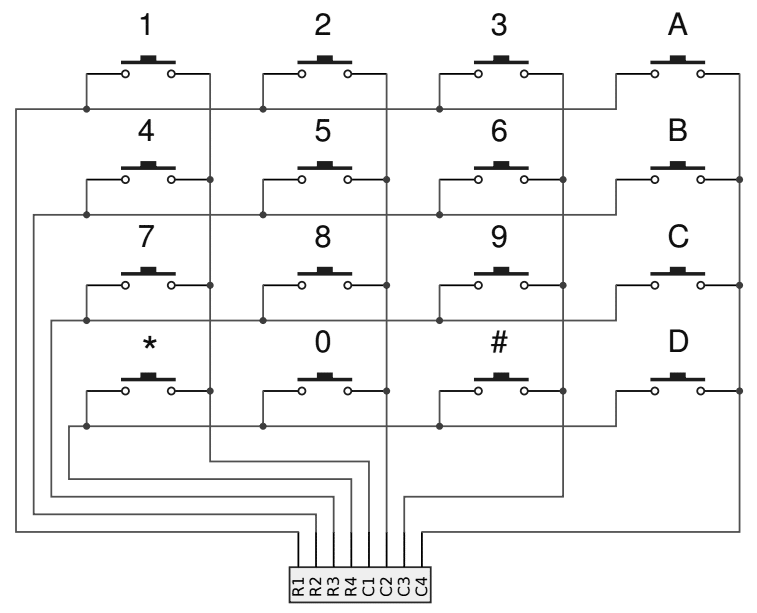
\includegraphics[width=0.6\textwidth]{images/4x4-keypad.png}
    \label{fig:schematic}
\end{figure}

\subsection{Pinbelegung des Arudinos}

Das 4x4 Tastenfeld und die RGB LED werden mit dem Arduino über folgende GPIO Pins verbunden:
\begin{lstlisting}[style=CStyle]
const int Output[rows]={2,3,4,5};
const int Input[columns]={6,7,8,9};
const int redPin = 10;
const int greedPin = 11;
const int bluePin = 12;
\end{lstlisting}

Dabei werden GPIO Pin 2 bis 5 als digitaler Output festgelegt. Diese Pins entsprechen R1 bis R4 des Tastenfelds. GPIO 6 bis 9 sind als digitaler Input eingestellt und entsprechen C1 bis C4. GPIO Pin 10 bis 12 sind digitale Ausgänge um die Intensität der jeweiligen Farben einzustellen.

\subsection{Versuchsaufbau}

Abbildung \ref{fig:sketch} ist der Sketch des Zahlenschlosses. Hierbei sind der Arduino-Uno, die RGB-LED, die Vorwiderstände und das Tastenfeld korrekt verbunden. Dabei stimmen die Pin-Belegungen mit dem aus dem Quellcode verwendeten Pins überein. 

\begin{figure}[H]
    \caption{Sketch des Zahlenschlosses}
    \centering
    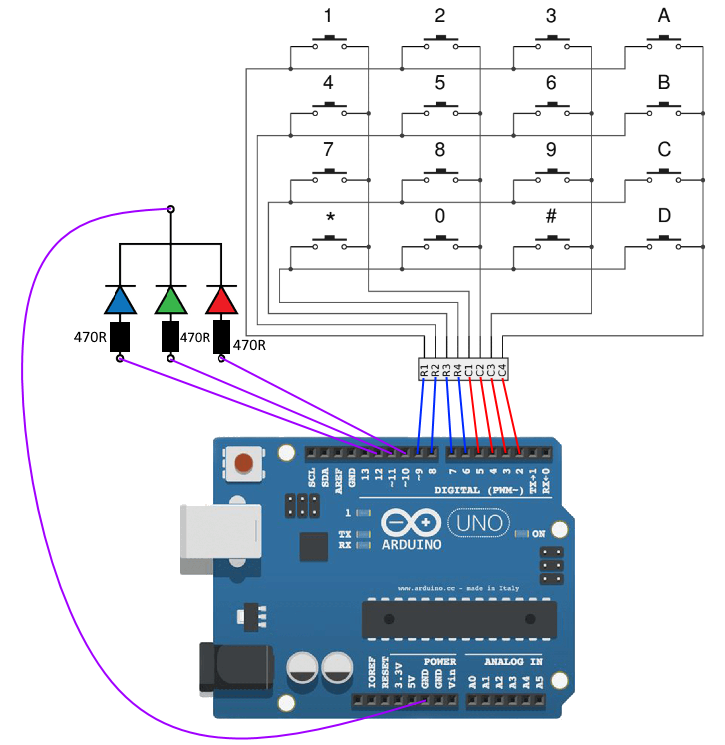
\includegraphics[width=0.7\textwidth]{images/sketch.png}
    \label{fig:sketch}
\end{figure}

\subsection{Zustandsmaschine}

Das Verhalten des Nummernschlosses wird als eine Zustandsmaschine beschrieben, welche in Abbildung \ref{fig:M1} zu sehen ist. Die PIN und der PUK werden im Quellcode fest definiert. Der Zustand 'init' ist der Startzustand der Maschine. Sobald eine Taste gedrückt wird, wechselt der Zustand in 'key'. Hierbei werden die Eingaben mitgezählt, bei der korrekten Eingabe einer Stelle wird der Zähler erhöht ('right key'). Ist die Eingabe falsch, wird zurück in den 'init' Zustand gewechselt und die Eingabe zurückgesetzt. Nach 4 Fehleingaben wird das Schloss gesperrt und von 'key' in den Zustand 'locked' gewechselt. Dieser Zustand kann nur verlassen werden, wenn die PUK korrekt eingegeben wird. Ist die PIN korrekt, wird in den Zustand 'open' gewechselt und das Schloss ist geöffnet. Hierbei kann der PIN geändert werden oder das Schloss sperrt sich nach einer gewissen Zeitspanne automatisch und wechselt in den Zustand 'init'. Falls eine PIN-Änderung gewünscht wird, muss eine bestimmte Zeichenfolge eingegeben werden. Nach der Aufzeichnung der Eingaben wird der neue PIN gespeichert und es wird zurück in den 'open' Zustand gewechselt. 

\begin{figure}[H]
\caption{Zustandsmaschine der Schlosssteuerun} \label{fig:M1}
\centering
    \begin{tikzpicture}[shorten >=1pt,node distance=3cm,on grid]
      \node[state,initial]   (init)                {init};
      \node[state]           (key) [right=of init] {key};
      \node[state]           (locked) [right=of key] {locked};
      \node[state]           (open) [right=of locked] {open};
      \node[state]           (change) [right=of open] {change};
      \path[->] (init)   edge   node [below] {input} (key)
                (key)    edge  [bend right]  node [above]   {wrong input} (init)
                         edge  [bend left]  node [above]   {correct pin} (open)
                         edge  [loop below]  node           {right key} ()
                         edge  node [below] {tries > 4} (locked)
                (locked) edge  [bend left=75]  node [below] {unlock with puk} (init)
                (open)   edge  [bend left]  node [above] {input} (change)
                         edge  [bend right=75]  node [below] {timeout} (init)
                (change) edge  [loop below]  node {key input} ()
                         edge [bend left=45] node [below] {change command} (open);
    \end{tikzpicture}
\end{figure}

Die Abbildung \ref{fig:usecase} ist ein Anwendungsfalldiagramm für die Schlosssteuerung. Hierbei gibt es zwei Gruppen von Anwendern. Die erste Gruppe sind die nutzenden Personen ('Employee'), welche die Tür entsperren wollen um durchzugehen. Diese benötigen hierfür einen PIN. Die zweite Gruppe sind die Administratoren, welche sich um die Verwaltung kümmern. Die Administratoren können gesperrte Schlösser mit der Hilfe eines PUK entsperren. Zusätzlich können sie den PIN ändern, wenn das Schloss offen ist und sie einen Befehl auf dem Tastenfeld eingeben. 

\begin{figure}[H]
    \caption{Use-Case Diagramm}
    \centering
    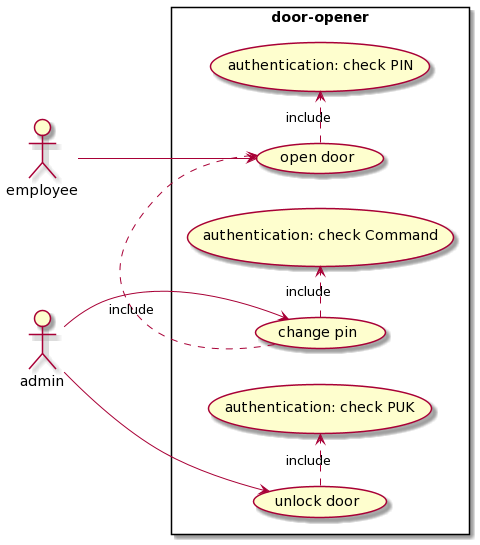
\includegraphics[width=0.5\textwidth]{images/usecase.png}
    \label{fig:usecase}
\end{figure}

In Abbildung \ref{fig:sequence-user} wird eine Sequenz von nutzenden Personen ('Employee'), Türschloss ('Keypad') und Tür ('Door') gezeigt. Zum besseren Verständnis wurde die Tür als Objekt noch zusätzlich eingefügt, auch wenn diese nicht im Aufbau erklärt wird. Möchte die nutzende Person die Tür öffnen gibt es zwei Fälle. Wenn das Schloss nicht gesperrt ist, kann die nutzende Person einen PIN eingeben um die Tür zu entsperren. Dabei werden die Antworten des Türschlosses als Farben auf der LED visualisiert (siehe Kapitel \ref{state-colors}). Ist die Tür gesperrt, kann die nutzende Person zwar das Tasten klicken aber das Schloss wird nicht reagieren.

\begin{figure}[H]
    \caption{Sequenzdiagramm - nutzende Person}
    \centering
    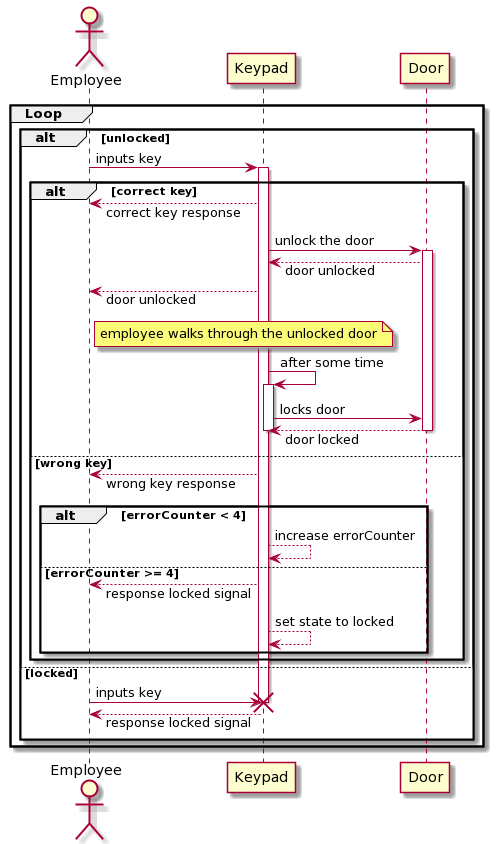
\includegraphics[width=0.6\textwidth]{images/sequence-user.png}
    \label{fig:sequence-user}
\end{figure}

Nun wird in der Abbildung \ref{fig:sequence-admin} die Sequenz von administrierenden Personen ('Admin') und dem Türschloss beschrieben. Dabei wird auf die Möglichkeit eingegangen das Schloss zu entsperren, falls der PIN zu oft falsch eingegeben wurde. Zusätzlich wird auch die Möglichkeit der Änderung des PIN beschrieben. In diesem Fall muss das Türschloss bereits über den PIN geöffnet worden sein. Auch hier werden die Antworten des Türschlosses mit Hilfe der LED visualisiert (siehe Kapitel \ref{state-colors}).

\begin{figure}[H]
    \caption{Sequenzdiagramm - Administrator}
    \centering
    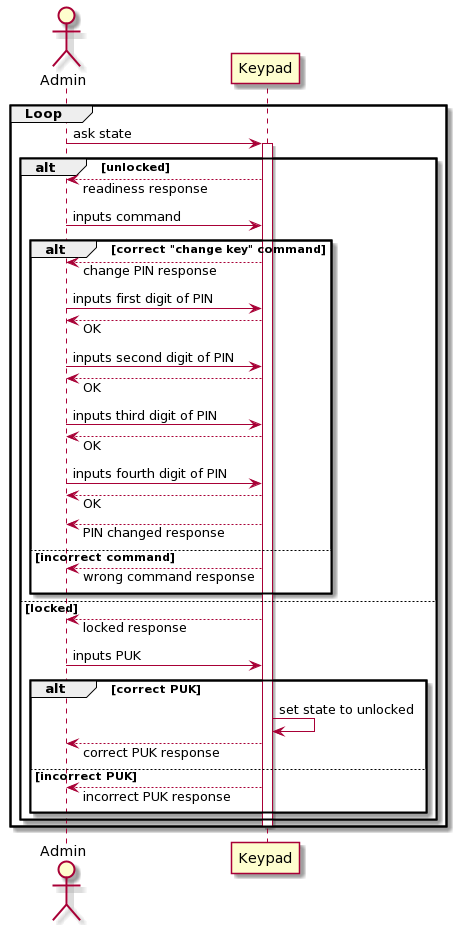
\includegraphics[width=0.6\textwidth]{images/sequence-admin.png}
    \label{fig:sequence-admin}
\end{figure}        

    \section{Einrichtung der Entwicklungsumgebung}
        Um das Programm auf den Mikrocontroller zu übertragen müssen folgende Bibliotheken installiert werden: 

\begin{itemize}
    \item binutils : um Werkzeuge wie Assembler, Linker zu bekommen
    \item gcc-avr : ein GNU C Cross-Compiler für speziell für AVR
    \item avr-libc: es ist ein Paket für AVR C Bibliotheken
    \item AVRDUDE : Anwendung zum programmieren des Mikrocontrollers
\end{itemize}

Darüber hinaus wird ein Makefile benutzt um den Programmcode zu kompilieren und den Mikrocontroller zu programmieren. Für den AVR-GCC Compiler werden noch spezielle Bibliotheken benötigt, diese können mit folgenden Befehlen installiert werden (Linux-Ubuntu) \cite{online:avrboard}:

\begin{lstlisting}[style=CStyle]
sudo apt-get install gcc-avr binutils-avr avr-libc
sudo apt-get install avrdude
\end{lstlisting}

Die AVR-GCC Toolchain kennt das Layout des Arduino Uno nicht, weswegen der konkrete Mikrocontroller richtig angesprochen werden muss. Im Speziellen ist auf dem Arduino Uno der Atmega328p verbaut. Dieser muss dann im Makefile angegeben werden, sodass der Programmcode für den Mikrocontroller passend kompiliert wird. 

Als Makefile wird eine abgeänderte Version des von Prof. Pretschner bereitgestellte Makefiles verwendet. So muss die MCU Angabe auf 'atmega328p' geändert, und die Angabe des Programmer für den AVRDUDE muss zu 'arduino' verändert werden. Abhängig davon, wie der Controller angeschlossen ist, muss zudem der Port in den AVRDUDE Einstellungen angepasst werden z. B. '/dev/ttyUSB0'.



    \section{Implementierung und Umsetzung}
        Der Programmcode ist modular aufgebaut. Sowohl die Zustandsmaschiene ('states.c') also auch das Tastenfeld ('keypad.c') und die LED-Steuerung ('led.c') sind in separaten Dateien getrennt. Im folgenden werden die Module kurz erklärt.

Jedes C-Programm, enthält die Definition einer Funktion namens 'main', die den designierten Start des Programms bzw den Programmeinstieg darstellt. Die 'main' Funktion wird, wie in diesem Fall, meist in einer Datei namens 'main.c' deklariert. In dieser Funktion werden die Pins jeweils für das Keypad und die LED eingestellt (Zeilen 8-9). Nach der Einstellung und der Initialisierung folgt eine Endlos-Schleife, welche die Zustandsmaschine ausführt (Zeilen 13-19). Hierbei wird eine kleine Verzögerung eingestellt um den Tastendruck optimal zu erfassen. Hierfür wird der millis timer benutzt welcher vor der schleife initialisiert wird und mit \textit{sei();} werden Interrupts aktivieren. 

\begin{lstlisting}[style=CStyle-numbers]
int main(void)
{
    setup_LED();
    setup_keypad();
    init_millis(16000000UL); //frequency the atmega328p is running at
    sei();
	
    while(1) //Infinite loop
    {
        if(millis()-kdelay>period) //used to make non-blocking delay
        {
            kdelay=millis();  //capture time from millis function
            stateM();
        }
    }
    return 0;
}
\end{lstlisting}

Die Zustandsmaschine wird in einem 'Switch-Case'-Block realisiert. Dieser wird in der Funktion 'stateM' ausgeführt. Und verändert anhand der Abbildung \ref{fig:M1} den Zustand. 
\begin{lstlisting}[style=CStyle]
void stateM()
{ ... }
\end{lstlisting}

Dabei haben die Zustände zur Visualisierung verschiedene Farben, welche per LED visualisiert werden. Hierbei wird die Funktion 'setLED(r, g, b)' benutzt, welche die jeweiligen Farben ansteuert, die im folgenden aufgeschlüsselt werden: 

\begin{itemize}
\label{state-colors}
    \item LOCKED: Rot
    \item NEWKEY: Gelb
    \item OPEN: Magenta
    \item KEY: Weiß
    \item INIT: Blau
    \item Gedrückte Taste: kurzes Grün
\end{itemize}

Innerhalb dieser Methode wird die Funktion 'keypad' aufgerufen, welche für das Erfassen der Tastendrücke zuständig ist. Dabei wird zuerst geprüft ob bereits eine Taste gedrückt wird, ist dies nicht der Fall wird auf einen Tastendruck geprüft. Wenn eine Spalte LOW ist wird auf die Zeile geprüft ob diese High ist. Wenn Zeile und Spalte identifiziert sind, konnte die Taste identifiziert werden und wird zurückgegeben.

\begin{lstlisting}[style=CStyle]
char keypad()
{ ... }
\end{lstlisting}

\noindent Abbildung \ref{fig:pic} zeigt den konkreten Versuchsaufbau des oben vorgestellten Schaltplans von Abbildung \ref{fig:sketch}. Die LED mit den Vorwiderständen wurden auf ein sog. 'Breadboard' gesteckt.

\begin{figure}[H]
    \caption{Versuchsaufbau des Schaltplans}
    \centering
    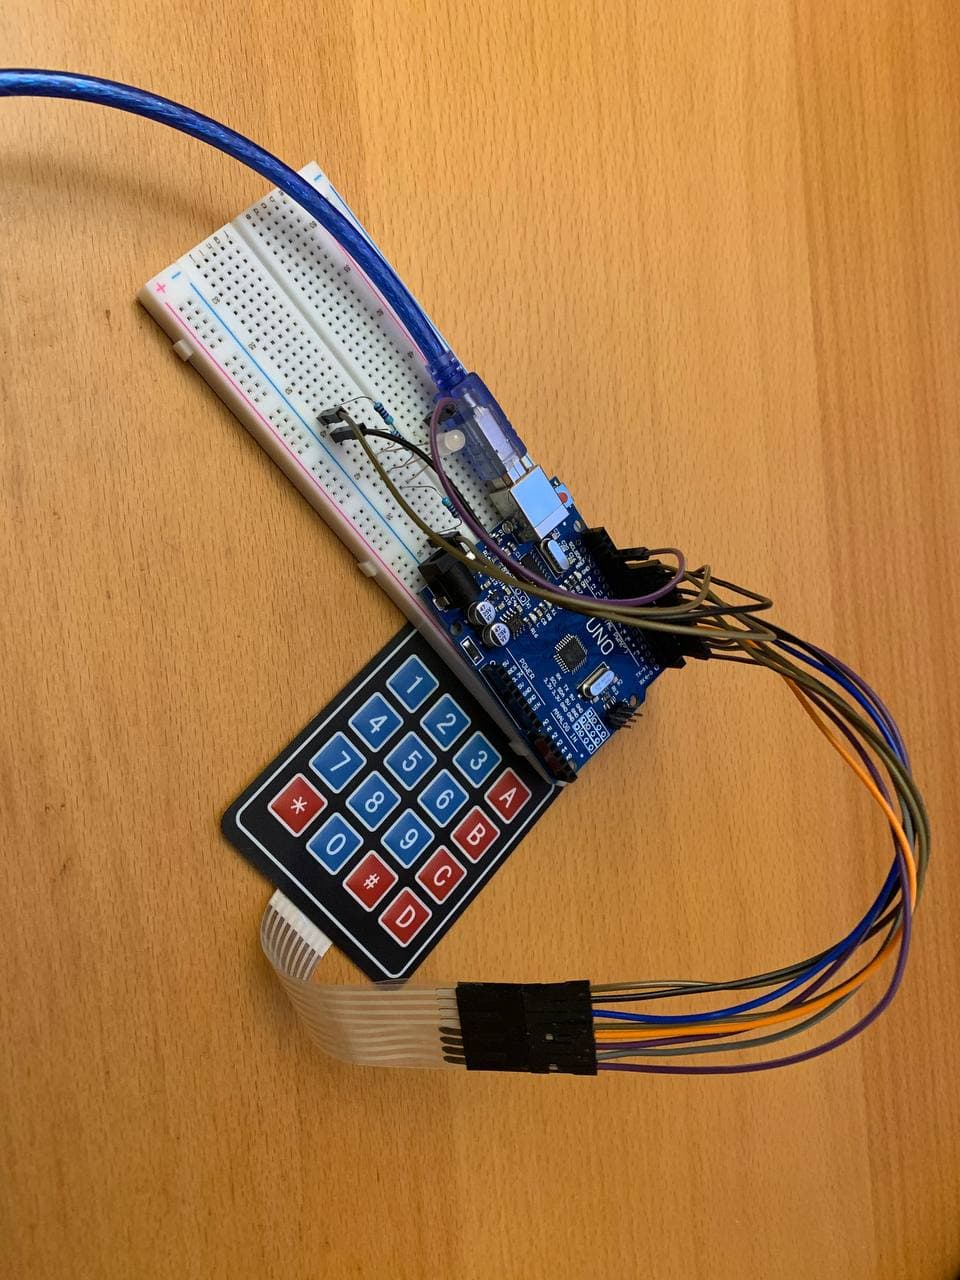
\includegraphics[width=0.6\textwidth]{images/picture.jpg}
    \label{fig:pic}
\end{figure}
    
    \section{Bedienungsanleitung}
        Sobald das Gerät mit Strom versorgt wird, kann die Schlosssteuerung benutzt werden. Hierfür visualisiert das grüne Leuchten der LED, dass die Schlosssteuerung korrekt gestartet wurde und auf einen Tastendruck wartet. Die Initial-PIN für das Entsperren des Schlosses lautet 'a123'. Dieser kann nach korrekter Eingabe geändert werden. Wenn eine Taste gedrückt wird, leuchtet die LED kurz Gelb auf um den Tastendruck zu bestätigen. Bei Misserfolg wird das Schloss zurückgesetzt und die vollständige PIN muss nochmals eingegeben werden. Wurde die PIN korrekt eingegeben wird das Schloss freigegeben und die LED leuchtet dauerhaft grün. Hier gibt es nun die Möglichkeit, die PIN zu ändern. Mit der Tastenkombination '\#a' im freigegebenen Schloss kann das Ändern der PIN initiiert werden. Nun leuchtet die LED Türkis und eine neue 4-stellige PIN kann eingegeben werden. Nach der Eingabe der neuen PIN wechselt das Schloss wieder in den geöffneten Modus. Nach einem kurzen Zeitintervall ohne Benutzereingabe wird das Schloss wieder geschlossen und die PIN muss erneut eingegeben werden. Sollte der PIN dreimal falsch eingegeben worden sein, wird das Schloss gesperrt und muss mit einem PUK entsperrt werden. Der PUK für das Entsperren lautet '\#12345'. Dieser kann beliebig oft eingegeben werden und erst bei erfolgreicher Eingabe wird das Schloss entsperrt.
    
    \section{Fazit}
        Eine Zustandsmaschine ist für ein kleines System eine passende Vorgehensweise. Für komplexere Systeme sollte eine andere Art von der Beschreibung des Systems gewählt werden, da für jeden Zustand ein neuer Wert definiert werden muss und dieser in das 'Switch-Case Statement' eingefügt werden muss. Dies führt bei komplexeren Systemen zu einer Verschlechterung der Code-Qualität und einem unleserlicheren Quellcode. Der Aufgabenstellung konnte entsprochen werden. So wurde ein Nummernschloss entworfen, welches entsprechend der Zustandsmaschine arbeitet und diese Zustände angemessen visualisiert. Auch wurde das Makefile so verändert, dass diese für den benutzen Mikrokontroller (Arduino Uno - ATMega328p) benutzt werden konnte.

Die Verwendung der Open-Source-Software 'Arduino-IDE' \footnote{\url{https://github.com/arduino/Arduino}} wäre aufgrund von weitreichender Unterstützung von Arduino-Mikrocontrollern eine bessere Entscheidung gewesen als die 'Eclipse'-IDE. So gab es am Anfang Probleme bei der Einrichtung der Entwicklungsumgebung, sowie Unstimmigkeiten bei einigen Funktionen. Dennoch konnte die IDE 'Eclipse' für dieses Projekt benutzt werden um den Quellcode zu erarbeiten und ein Makefile zu erstellen, sowie zum Hochladen der Anwendung auf den Mikrocontroller.


    
    \newpage
    
    \pagenumbering{Roman}
    \appendix
    
    \section*{Literaturverzeichnis}
    \addcontentsline{toc}{section}{\protect\numberline{}Literaturverzeichnis}%
        \printbibliography
    
    \newpage
    
    \addcontentsline{toc}{section}{\protect\numberline{}Abbildungsverzeichnis}%
        \listoffigures

\end{document}